\section{Matrix Factorization Model}
\label{sec:model} This section will  present the matrix
factorization model which is used for outlier detection. Before
discussing the model in detail, we present the notations and
definitions.  We represent the corpus of text documents as a bag of
words matrix.  A lowercase or uppercase letter such as $x$ or $X$,
is used to denote a scalar. A boldface lowercase letter, such as
$\mathbf{x}$, is used to denote a vector, and  a boldface uppercase
letter, such as $\mathbf{X}$, is used to denote a matrix. This is
consistent with what is commonly used in much of the data mining
literature. Indices typically start from $1$, unless otherwise
mentioned.  For a $\mathbf{X}$, $\mathbf{x}_{i}$ denotes its
$i^{th}$ column, $\mathbf{y}_j^\intercal$ denotes its $j^{th}$ row
and $x_{ij}$ or $X(i,j)$ or $(X)_{ij}$ denote its $(i,j)^{th}$
element.

For greater expressibility, we have also borrowed certain notations
from matrix manipulation scripts such as Matlab and Octave.  For
example, the notation $max(\mathbf{x})$ returns the maximal element
$x \in \mathbf{x}$ and $max(\mathbf{X})$ returns a vector of maximal
elements from each column $\mathbf{x} \in \mathbf{X}$. Similarly,
$\mathbf{X}(i,:)$ denotes the $i$-th row of the matrix and
$\mathbf{X}(:,i)$ for $i$-th column.  For the  reader's convenience,
the notations  used in the paper are summarized in  Table
\ref{table:notations}.

Let $\mathbf{A}$ be the matrix representing the underlying data. In
the context of a text collection, this corresponds to a
term-document matrix, where terms correspond to rows and documents
correspond to columns. In other words, $a_{ij}$ denotes the number
of times the term $i$ appears in document $j$.  Generally, we
can write $\mathbf{A}$ as follows:
\begin{equation}
\mathbf{A} = \mathbf{L_0} + \mathbf{Z_0}.
\end{equation}

\begin{figure}
\scalebox{0.34}[0.29]{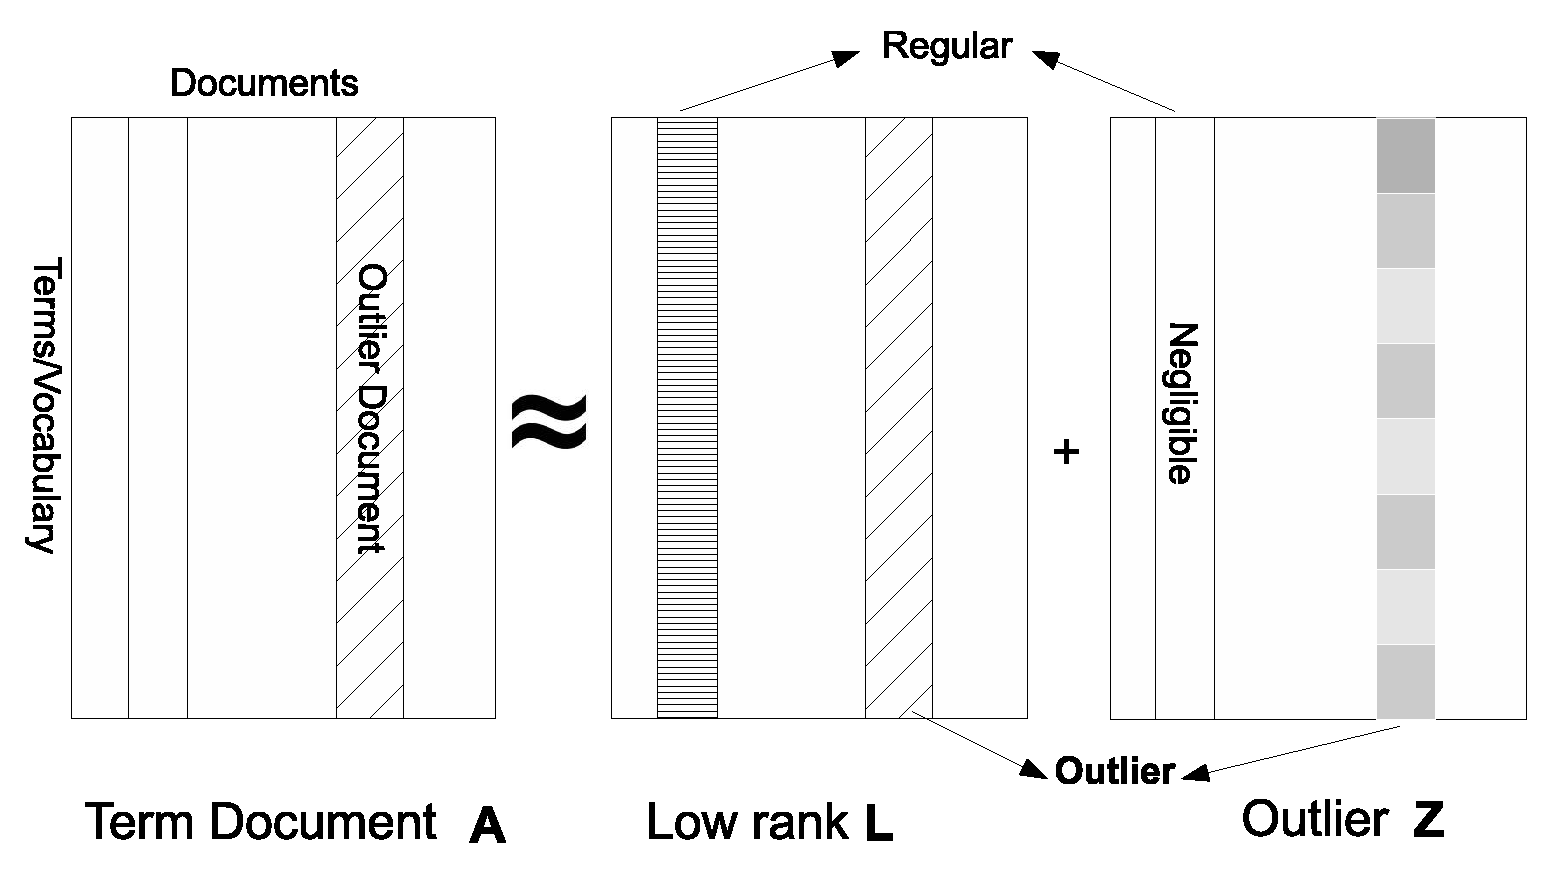
\includegraphics{outlieroverview.eps}}
\caption{Text Outliers Using NMF} \label{fig:outlieroverview}
\end{figure}

Here, $\mathbf{L_0}$ is  a low rank matrix and $\mathbf{Z_0}$
represents the matrix of  outlier entries. Typically, the matrix
$\mathbf{L_0}$ represents the documents created by a lower rank
generative process (such as that modeled by pLSI), and the parts of
the documents that do not correspond to the generative process are
represented as part of the matrix $\mathbf{Z_0}$.   In real world
scenarios, the outlier matrix $\mathbf{Z_0}$  contains  entries
which are very close to zero, and  only a small number of entries
have {\em significantly} non-zero values. These significantly
nonzero entries are often present in only a small fraction of the
columns. Columns which are fully representable in terms of factors
are consistent with the low rank behavior of the data, and therefore
{\em not} outliers. The rank of $\mathbf{L}_0$ is not known in
advance, and it can be expressed in terms of its underlying factors.
$$
\mathbf{L}_0 \approx \mathbf{W}_0\mathbf{H}_0
$$
Here, the two matrices   have dimensions $\mathbf{W}_0 \in
\mathbb{R}^{m \times r}_+$, $\mathbf{H}_0 \in \mathbb{R}^{r \times
n}_+$, and $r \le rank(\mathbf{L}_0)$. The matrices $\mathbf{W}_0$
and  $\mathbf{H}_0$ are non-negative, and this provides
interpretability in terms of being able to express a document as a
non-negative linear combination of the relevant basis vectors, each
of which in itself can be considered a frequency-annotated bag of
words (topics) because of its non-negativity.  Specifically,
$\mathbf{H_0}$ corresponds to the coefficients for the basis matrix
$\mathbf{W_0}$. Intuitively, this corresponds to the case that every
document
 $\mathbf{a}_i$, is represented as the linear combination of
the $r$ topics. In cases, where this is {\em not} true, the document
is an outlier, and those  unrepresentable sections of the matrix are
captured by the non-zero entries in the   $\mathbf{Z_0}$ matrix. In
real scenarios,  the entries in  this matrix are often  extremely
skewed, and the small number of non-zero entries very obviously
expose the outliers.  The decomposition of the matrix into different
component is pictorially illustrated  in Figure
\ref{fig:outlieroverview}.

In order to determine the best low rank factorization, one must try
to optimize the  aggregate  values of the residuals in  the matrix.
This can of course be done in a variety of ways, depending upon the
goals of the underlying factorization process.  We model the
determination of the matrices $\mathbf{W}$,$\mathbf{H}$, and
$\mathbf{Z}$, as the following optimization problem:
\begin{equation}\label{l12norm}
(\mathbf{W}_0,\mathbf{H}_0;\mathbf{Z}_0)=\argmin_{\mathbf{W}\ge0,\mathbf{H}\ge0; \mathbf{Z}}  \frac{1}{2}\norm{\mathbf{A}-\mathbf{W}\mathbf{H}-\mathbf{Z}}_F^2 + \alpha\norm{\mathbf{Z}}_{1,2}
\end{equation}

The specific location of outliers in each column does not have a
closed form solution, since the $\ell_{1,2}$-norm penalty is applied
to $\mathbf{Z}$.   The   logic for applying the $\ell_{1,2}$-norm in
the context of the outlier detection problem is as follows.  Each
entry in the $\mathbf{Z}$ corresponds to a term in a document,
whereas we are interested in the outlier behavior of entire
document. This aggregate outlier behavior of the document $x$ can
be modeled with the $\ell_2$ norm score of a particular column
$\mathbf{z}_x$. In a real scenario,  if a large segment  of a
document $x$ is not representable as the linear combination of the
$r$ topics through $\mathbf{L_0}$, the corresponding column
$\mathbf{z}_x$ in the matrix $\mathbf{Z}$ will be compensated by
having more entries in its column.  In other words, we will  have a
higher $\ell_2$ value for the corresponding column $\mathbf{z}_x$,
and this corresponds to a higher outlier score.
 Furthermore, the  $\ell_{1,2}$-norm penalty on $\mathbf{Z}$
defines the sum of the $\ell_2$ norm outlier scores over all the
documents.  Therefore,  the optimization problem essentially tries
to find the best model,  an important component of which is to
minimize the sum of the outlier scores over all documents.  While a
variety of different  (and more commonly used) penalties such as the
Frobenius norm are available for matrix factorization models, we
have chosen the $\ell_{1,2}$-norm penalty because of its intuitive
significance in the context of the outlier detection problem, and
its tendency to create skewed outlier scores across the columns of
the matrix. As we will see in the next section, this comes at the
expense of a formulation which is more difficult to solve
algorithmically.

For high dimensional data, sparse coefficients are desirable for
obtaining an interpretable low rank matrix $\mathbf{W}\mathbf{H}$.
For this purpose, we add the $\ell_1$-penalty on $\mathbf{H}$:
\begin{equation}\label{outlier}
\min_{\mathbf{W}\ge0,\mathbf{H}\ge0; \mathbf{Z}}  \frac{1}{2}\norm{\mathbf{A}-\mathbf{W}\mathbf{H}-\mathbf{Z}}_F^2 + \alpha\norm{\mathbf{Z}}_{1,2} + \beta\norm{\mathbf{H}}_{1}
\end{equation}
 The constant $\alpha$ defines the weight
for the outlier matrix $\mathbf{Z}$ over the recovery of the low
rank space $\mathbf{L}$ and the sparsity term. In the case of
outlier detection in text documents, we give more weight for the
outlier matrix over the low rank representation $\mathbf{L}$. This
problem does not have a closed form solution, and
 therefore we cannot  directly recover the low rank
matrix $\mathbf{W}\mathbf{H}$ in closed form. However, we can
recover the column space. Without non-negativity constraints, this
property is also known as the rotational invariant property
\cite{ding06,xu12}. This particular formulation of the matrix
factorization model is a bit different from the commonly used
formulations, and off-the-shelf solutions do not directly exist for
this scenario. Therefore, in a later section, we will carefully
design an algorithm with the use of block coordinate descent for
this problem.

In order to understand the modeling of the outliers better, we
present the readers with a toy example from a real world data set,
to show how  skewed the typical values of the corresponding column
$\mathbf{z}(x)$ may be in real scenarios.  In this case, we used the
{\em BBC} dataset\footnote{\url{http://mlg.ucd.ie/datasets/bbc.html}}.
\ramki{This dataset consists of documents from BBC news website corresponding
to stories in area business, entertainment, politics, sport, tech from 2004-2005 . 
%We ran our algorithm \algo explained in the next Section
%\ref{sec:algorithm} to find the matrices $\mathbf{W,H}$ and $\mathbf{Z}$.
We took all the documents from business and politics  and 50
documents from tech labeled as outliers. We randomly permuted the columns to 
shuffle the outliers in the matrix to avoid any spatial bias}. 
We computed the $\mathbf{Z}$ matrix
and   generated the $\ell_2$ scores of the columns of outlier matrix
$\mathbf{Z}$. Figure \ref{fig:outlierz} shows the outlier($\ell_2$)
scores of the documents. The $X$-axis illustrates the index of the
document, and the $Y$-axis illustrates the outlier score. It is
evident that  the scores for some  columns are so close to zero,
that they cannot even be seen on the diagram drawn to scale. These
columns also happened to be the non-outlier/regular documents of the collection.
Such documents $\mathbf{a}_x \in \mathbb{R}^m$ correspond to the low
rank space, and  are approximately representable as  a product of
the basis  matrix $\mathbf{W}$ with the corresponding column vector
of coefficients $\mathbf{h}_x \in \mathbb{R}^r$ drawn from
$\mathbf{H}$. However, the documents that are not representable in
such a low rank space have a large outlier score. From the
distribution of the outlier score, we can also observe that the
scores of outlier documents against non-outliers are clearly
separable, by using a simple statistical mean and standard deviation
analysis. Therefore, while we use the scores to rank the documents
in terms of their outlier behavior, the skew in the entries ensures
that it is often easy to choose a cut-off in order to distinguish
the outliers from the non-outliers.

\begin{figure}
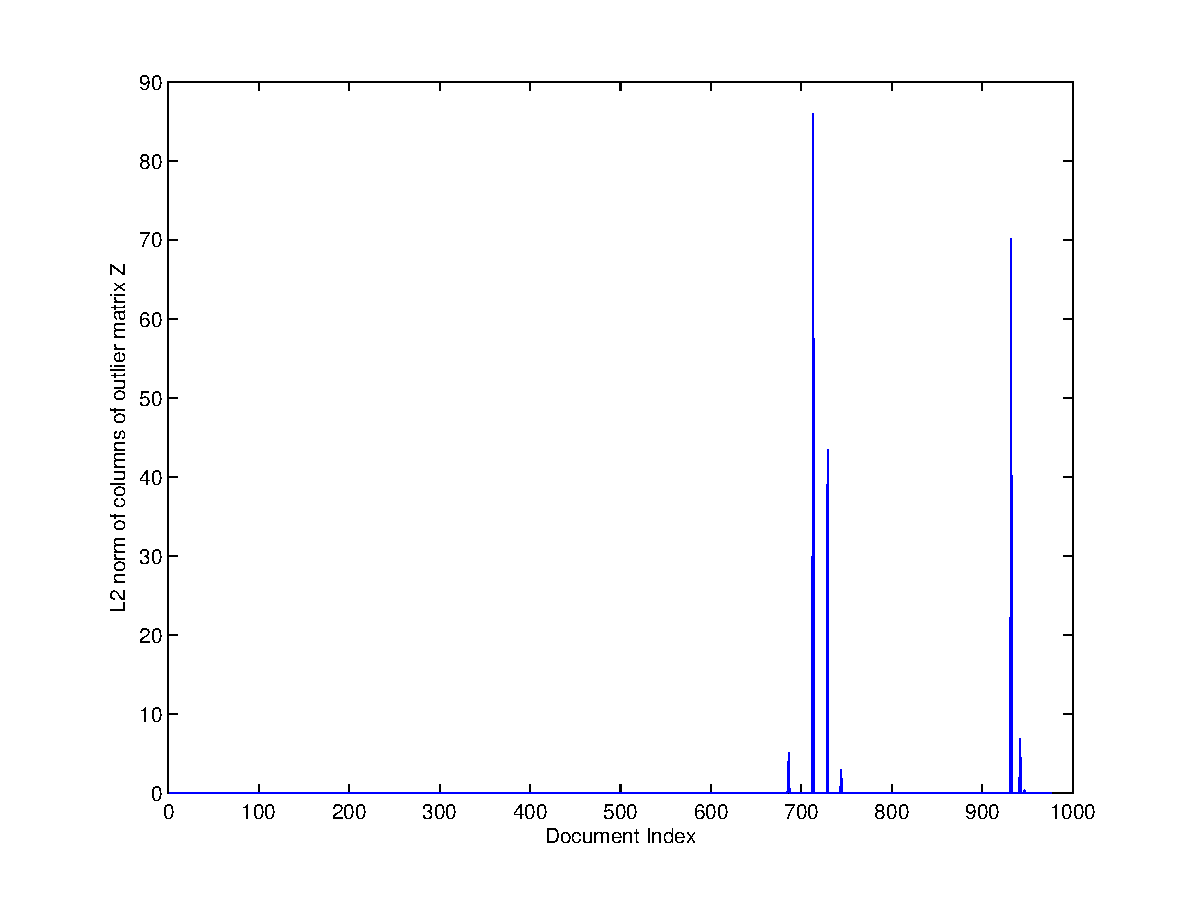
\includegraphics[scale=0.4]{outlierzbbc.eps}
\caption{$\ell_2$ norm of columns of $\mathbf{Z}$ outlier matrix}
\label{fig:outlierz}
\end{figure}



In the following sections, we will analyze the property and
performance of this model \eqref{outlier} for outlier detection
problems.
